\documentclass{article} % For LaTeX2e
\usepackage{nips14submit_e,times}
\usepackage{hyperref}
\usepackage{url}

\usepackage[leqno, fleqn]{amsmath}
\usepackage{amssymb}
\usepackage{qtree}
\usepackage[numbers]{natbib}
\usepackage{graphicx}


\renewcommand{\bibsection}{\subsubsection*{\bibname}}

\usepackage{gb4e}
\newcommand{\natneg}{\raisebox{2px}{\tiny\thinspace$\wedge$\thinspace}}
\def\ii#1{\textit{#1}}

\title{DRAFT: Learning to represent abstract structures for natural language reasoning}

\author{
Samuel R. Bowman \\
NLP Group, Dept. of Linguistics\\
Stanford University\\
Stanford, CA 94305-2150 \\
\texttt{sbowman@stanford.edu}
 \And
 Christopher Potts \\
Dept. of Linguistics\\
Stanford University\\
Stanford, CA 94305-2150 \\
\texttt{cgpotts@stanford.edu}
 \And
Christopher D. Manning \\
NLP Group,  Depts. of Computer Science and Linguistics\\
Stanford University\\
Stanford, CA 94305-2150 \\
\texttt{manning@stanford.edu}
}

\newcommand{\fix}{\marginpar{FIX}}
\newcommand{\new}{\marginpar{NEW}}

% \nipsfinalcopy % Uncomment for camera-ready version

\begin{document}
\maketitle

% TODO: Insert results
% TODO: Standardize first person pronouns

\begin{abstract}
Supervised recursive neural network models (RNNs) for sentence meaning
have been successful in a wide array of sophisticated language tasks,
but it remains an open question whether they can achieve the same
results as compositional semantic grammars based in logical forms. We
address this question directly by using a logical grammar to generate
controlled data sets encoding the relationships (entailment, synonymy,
contradiction) between pairs of expressions and evaluating whether
each of two classes of neural model --- plain RNNs and recursive
neural tensor networks (RNTNs) --- can learn those relationships
correctly. Our first experiment confirms that both models can learn
the basic algebra of logical relations involved. Our second and third
experiments expand on this result to cover complex recursive
structures and sentences involving quantification. We find that the
plain RNN achieves only mixed results on the first and second
experiments, but that the stronger RNTN models generalized well in
every case. % TODO: Update to reflect results
\end{abstract}
\section{Introduction}\label{sec:intro}

% TODO: Earlier work on NN interpretation \cite{Garcez-etal:2001}

Supervised recursive neural network models (RNNs) for sentence meaning
have been successful in a wide array of sophisticated language tasks,
including sentiment analysis, analogy completion, image description,
and paraphase detection. These results are encouraging about the
ability of these models to learn compositional semantic grammars, but
it remains an open question whether they can achieve the same results
as grammars based in logical forms when it comes to core semantic
concepts like quantification, entailment, and contradiction defined
over complex linguistic structures. These concepts are central to
robust natural language understanding, so it is essential that our
computational models be able to capture them.

We address this question directly by using a logical grammar to
generate controlled data sets encoding the semantic relationships
between pairs of expressions and evaluating whether each of two
classes of neural model --- plain RNNs and recursive neural tensor
networks (RNTNs) --- can learn those relationships correctly. Our
logical grammar is a version of the natural logic developed by
\cite{maccartney2009extended}, which defines seven core relations of
synonymy, entailment, contradiction, and mutual consistency. Natural
logic is well-suited to our purposes because of it defines a rich set
of relations between words, phrases, and sentences, and because its
logical expressions are derived directly from surface forms, making it
amenable to large-scale natural language processing.

In our first experiment, we show that both of these models can learn
the core relational algebra of natural logic from data. Our second
experiment builds on this result to cover relations between complex
recursive structures like `(A or B)' and `not(not A and not B)', and
our third experiment involves relations between quantified statements
like `every reptile walks' and `every turtle moves'. We find that the
plain RNN achieves only mixed results on the second and third
experiments, but that the stronger RNTN models generalized well in
every case, suggesting that it has in fact learned, or at least
learned to simulate, our target logical concepts. % TODO: Update with current results

Citations to additional past work to be added.\\...\\...\\...\\...\\...\\...\\...\\...\\...\\...

% Deep learning methods in NLP which learn vector representations for words have seen successful uses in recent years on increasingly sophisticated tasks \cite{collobert2011natural, socher2011semi, socher2013acl1, chen2013learning}. Given the still modest performance of semantically rich NLP systems in many domains---question answering and machine translation, for instance---it is worth exploring the degree to which learned vectors can serve as general purpose semantic representations. Much of the work to date analyzing vector representations for words (see \cite{baroni2013frege}) has focused on lexical semantic behaviors---like the similarity between words like \ii{Paris} and \ii{France}. Good similarity functions are valuable for many NLP tasks, but there are real use cases for which it is necessary to know how words relate to one another or to some extrinsic representation, and to model the ways in which word meanings combine to form phrase, sentence, or document meanings. This paper explores the ability of linguistic representations developed using supervised deep learning techniques to support interpretation and reasoning. 

% TODO: Name RNTNs

% There are two broad family of tasks that could be used to test the ability of a model to develop general purpose meaning representations. In an interpretation task, sentences are mapped onto some denotation, such as  \ii{true} or \ii{false} for statements, or a factual answer for questions. There has been preliminary work in developing distributed models for interpretation \cite{grefenstette2013towards, rocktaschellow}, but developing a representation of world knowledge that corresponds accurately to the content expressed in language introduces considerable design challenges. I approach the problem by way of an inference task instead. Inferring the truth of one sentence from another does not require any preexisting knowledge representations, but nonetheless requires a precise representation of sentence meaning. I borrow the structure of the task from MacCartney and Manning  \cite{maccartney2009extended}. In it, the model is presented with a pair of sentences, and made to label the logical relation between the sentences as equivalence, entailment, or any of five other classes, as here:

%\begin{quote}
%\begin{enumerate}\small
%\item Many smartphone users avoid high bills overseas by disabling data service.
%\item Not everyone uses their smartphones for email when traveling abroad.
%\end{enumerate} 
%$\Rightarrow$ Entailment
%\end{quote}

%In this paper, we test the ability of recursive models to on three simple tasks, each of which is meant to capture a property that is necessary in representing natural language meaning in the setting of inference. I begin with an overview of MacCartney and Manning's \cite{maccartney2009extended} framework for inference, and of the recursive neural networks that I study. by showing that these models can learn to correctly represent entailment representations between sentences. I then show that these models can capture the meanings of recursive structurers accurately up to a sufficient depth. I finally close with a brief demonstration of the ability of these models to reason over short natural language sentences involving quantifiers. 

% TODO: Cite ICLR paper, emphasize new work since

\subsection{The task: natural language inference}

% TODO: cite \cite{watanabe2012latent} for past work on ML for McC&M-style NLI

% Condense?
In the standard formulation of the inference task (and the one used in the RTE datasets \cite{dagan2006pascal}), the goal is to determine whether a reasonable human would infer a hypothesis from a premise.
MacCartney formalizes a method of inferring entailment relations, and moves past two way entailment/non-entailment classification, proposing the set $\mathfrak{B}$ of seven labels meant to describe all of the possible non-trivial relations that might hold between pairs of statements, shown in Table \ref{b-table}. 

\begin{table}
\begin{center}
\begin{tabular}{|c|c|c|c|} \hline
name & symbol & set-theoretic definition & example \\ \hline \hline
entailment & $x \sqsubset y$ & $x \subset y$ & \ii{crow, bird}  \\ \hline
reverse entailment & $x \sqsupset y$ & $x \supset y$ & \ii{Asian, Thai}  \\ \hline
equivalence & $x \equiv y$ & $x = y$ & \ii{couch, sofa} \\ \hline
alteration & $x$ $|$ $y$ & $x \cap y = \emptyset \wedge x \cup y \neq \mathcal{D}$ & \ii{cat, dog} \\ \hline
negation & $x \natneg y$ & $x \cap y = \emptyset \wedge x \cup y = \mathcal{D}$ & \ii{able, unable} \\ \hline
cover & $x \smallsmile y$ & $x \cap y \neq \emptyset \wedge x \cup y = \mathcal{D}$ & \ii{animal, non-ape} \\ \hline
independence & $x$ \# $y$ & (else) & \ii{hungry, hippo}\\ \hline
\end{tabular}
\caption{The entailment relations in  $\mathfrak{B}$. $\mathcal{D}$ is the universe of possible objects of the same type as those being compared, and the relation \# applies whenever none of the other six do, including when there is insufficient knowledge to choose a label.}
\label{b-table}
\end{center}
\end{table}

% TODO: Reframe for updated experiments.
In order to minimize this possibility, I define the task of strict unambiguous NLI (SU-NLI). In this task, only entailments that are licensed by a strictly literal interpretation of the provided sentences are considered valid, and several constraints are applied to the language to minimize ambiguity:
\begin{itemize}
\ex A small, unambiguous vocabulary is used.
\ex All strings are given an explicit unlabeled tree structure parse.
\ex Statements involving the hard-to-formalize generic senses of nouns---i.e. \ii{dogs bark} as opposed to the non-generic \ii{all dogs bark}---are excluded.
\ex The sentences do not contain context dependent elements. This includes any reference to time or any tense morphology, and all pronouns.
\ex The morphology is dramatically simplified: the copula is not used (\ii{some puppy is French} is simplified to \ii{some puppy French}, to make it more directly comparable to sentences like \ii{some puppy bark}), and agreement marking (\ii{they walk} vs. \ii{she walks}) is omitted.
\end{itemize}

The key to success at this task is to learn a set of representations and functions that can mimic the logical structure underlying the data. There is limited precedent that deterministic logical behavior can be learned in supervised deep learning models: \citet{socher2012semantic} show in an aside that a Boolean logic with negation and conjunction can be learned in a minimal recursive neural network model with one-dimensional (scalar) representations for words. Modeling the logical behavior that underlies linguistic reasoning, though, is a substantially more difficult challenge, even in modular hand-built models.

The natural logic engine at the core of MacCartney's \cite{maccartney2009natural} NLI system requires a complex set of linguistic knowledge, much of which takes the form of what he calls projectivity signatures. These signatures are tables showing the entailment relation that must hold between two strings that differ in a given way (such as the substitution of the argument of some quantifier), and are explicitly provided to the model
for dozens of different cases of insertion, deletion and substitution of different types of lexical item. For example in judging the inference \ii{no animals bark $|$ some dogs bark} it would first used stored knowledge to compute the relations introduced by each of the two differences between the sentences. Here, the substitution of \ii{no} for \ii{some}  yields $\natneg$ and the substitution of \ii{dogs} for \ii{animals} yields $\sqsupset$. It would then use an additional store of knowledge about relations to resolve the resulting series of relations into one ($|$) that expresses the relation between the two sentences being compared:
\begin{quote}

1. \ii{no animals bark $\natneg$ \textbf{some} animals bark}\\
2. \ii{some animals bark $\sqsupset$ some \textbf{dogs} bark}\\
3. \ii{no animals bark $[\natneg\bowtie\thinspace\sqsupset\thinspace = |]$ some dogs bark}

\end{quote}

This study is the first that I am aware of to attempt to build an inference engine based on learned vector representations, but two recent projects have attempted to introduce vector representations into inference systems in other ways: 
\citet{baroni2012entailment} have achieved limited success in building a classifier to judge entailments between one- and two-word phrases (including some with quantifiers), though their vector representations were crucially based on distributional statistics and were not  learned for the task.
In another line of research, \citet{garrette2013formal} propose a way to improve standard discrete NLI with vector representations. They propose a deterministic inference engine (similar to MacCartney's) which is augmented by a probabilistic component that evaluates individual lexical substitution steps in the derivation using vector representations, though again these representations are not learned, and no evaluations of this system have been published to date.
\label{sec2}

% TODO: Mention all seven relations seen in all three experiments, but distribution uneven

\section{Recursive neural network models}

% TODO: Self cite.

The models that we study is are centered aronund a recursively applied composition function which is meant to mimic the recursive construction of meanings in formal semantics. In this scheme, pairs of words are merged into phrase representations by a function that maps from representations of length $2N$ to representations of length $N$. These phrase representations are then further merged with other words and phrases until the entire phrase or sentence being evaluated is represented in a single vector. This vector is then used as the input to a classifier and used in a supervised learning task.

Borrowing a model directly from the existing literature for this task is impossible since none has been proposed to detect asymmetric relations between phrases. Instead, we build a combination model, depicted in Figure \ref{sample-figure}. The two phrases being compared are built up separately on each side of the tree using the same composition function until they have each been reduced to single vectors. Then, the two phrase vectors are fed into a separate comparison layer that is meant to generate a feature vector capturing the relation between the two phrases. The output of this layer is then given to a softmax classifier, which in turn produces a hypothesized distribution over the seven relations.

For a composition layer, we experiment with both a plain neural network layer function (eq. \ref{rnn}) and the RNTN layer function proposed in \citet{chen2013learning} (eq. \ref{rntn}). A sigmoid nonlinearity (elementwise $\tanh$) is applied to the output of either layer function, following Socher et al.
\begin{gather} \label{rnn}
y_{RNN} = f(\mathbf{M} [\vec{x}^{(l)}; \vec{x}^{(r)}] + b_i)\\ % TODO: Add column vectors?
\label{rntn}
y_{RNTN} = f(\vec{x}^{(l)T} \mathbf{A}^{[1...N]} \vec{x}^{(r)} + \mathbf{B} [\vec{x}^{(l)}; \vec{x}^{(r)}] + \vec{c})
\end{gather} % TODO: Explain third order tensor parameter?

The comparison layer uses the same type of function with different parameters and a different nonlinearity function wrapped around it. Rather than use a $\tanh$ nonlinearity here, I found a substantial improvement in performance by using a rectified linear function for $f_{b}$. In particular, I use the leaky rectified linear function \cite{maasrectifier}: $f_{b}(\vec{x})=\max(\vec{x}, 0) + 0.01\min(\vec{x}, 0)$,  applied elementwise. 

To run the model forward and label a pair of phrases, the structure of the lower layers of the network is assembled so as to mirror the tree structures provided for each phrase. The word vectors are then looked up from the vocabulary matrix $V$ (one of the model parameters), and the composition and comparison functions are used to pass information up the tree and into the classifier at the top. The model is trained using backpropagation through structure  \cite{goller1996learning}, wherein the negative log of the probability assigned to the correct label is taken as a cost function, and the gradient of each parameter with respect to that cost function is computed at each node, with information passing down the tree and into both the function parameters and the vocabulary matrix. Gradients for different instances of the composition function or different instances of a word in the same tree are summed to produce at most a single gradient update per parameter.

\textit{Optimization:} I train the model with stochastic gradient descent (SGD), with gradients pooled from randomly chosen minibatches of 32 training examples, and learning rates computed using AdaGrad \cite{duchi2011adaptive} from a starting rate of 0.2. The parameters (including the vocabulary) are initialized randomly using a uniform distribution over $[-0.1, 0.1]$. % TODO: Update

\begin{figure}
\begin{center}
% \Tree [.{\sc softmax classifier}  [.{\sc comparison layer} [.{\sc \ii{dog} vector from $V$} ] [.{\sc composition layer} [.{\sc composition layer} [.{\sc \ii{very} vector from $V$} ] [.{\sc \ii{big} vector from $V$} ] ] [.{\sc \ii{cat} vector from $V$} ] ] ] ]
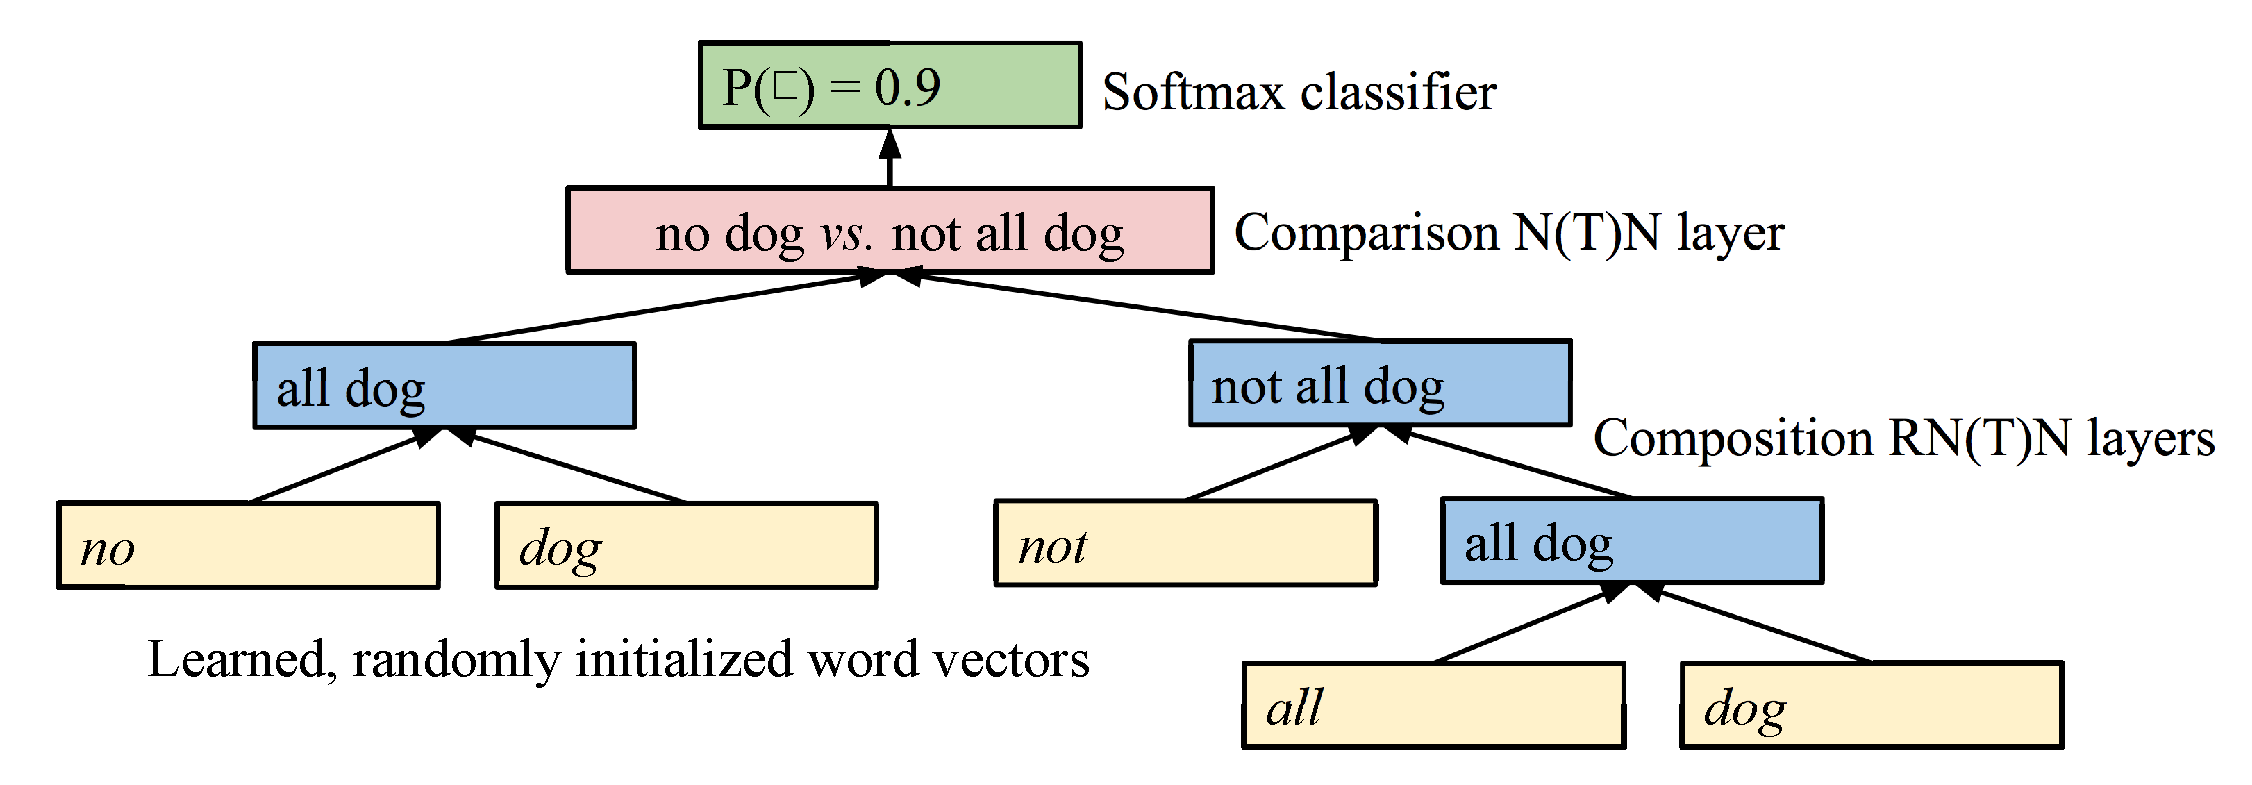
\includegraphics[scale=0.36]{model.eps}
\end{center}
\caption{The model structure used to compare \ii{no dog} and \ii{(not all) dog}. \label{sample-figure}} 
\end{figure}

\ii{Source code and data will be released after the conclusion of the review period.} % TODO: Or upon request? Attach anonymized code?

\section{Relation composition}

In order for a model to be able to learn to mimic the behavior of a relational logic like the one presented here from a finite amount data, it must be able to learn to deduce new relations from seen relations. The simplest such deductions involve facts about the relations themselves that do not involve considering the internal structure of the things being compared. For example, given that $a\sqsupset b$ and $b\sqsupset c$ one can conclude that $a\sqsupset c$ by the transitivity of $\sqsupset$, even without understanding $a$, $b$, or $c$. These seven relations support more than just transitivity: MacCartney and Manning's \cite{maccartney2009extended} join table defines 32 valid inferences that can be made on the basis of pairs of relations of the form $a R b$ and $b R' c$, including several less intuitive ones such as that if $a \natneg b$ and $b~|~c$ then $a \sqsupset c$. 

\begin{figure}[t]
\begin{center}
\begin{tabular}{ll|lll}
$a := \{1, 3, 4, 5, 6\}	$&~~~&~~~& $a \equiv a$	    	& $a~\#~c$	\\
$b := \{0, 3, 5, 6\}	$&~~~&~~~& $e \sqsupset c$	&$b \smallsmile c$		\\
$c := \{1, 2, 3, 4\}	$&~~~&~~~& $d \smallsmile e$	& $b~\#~d$		\\
$d := \{0, 4\}		$&~~~&~~~& $a \sqsubset e$	& $ d \equiv d$	\\
$e := \{1, 2, 3, 4, 5, 6\}$&~~~&~~~& $a~\#~b$		& ... 	\\
\end{tabular}
\end{center}

\caption{Some sample randomly generated sets, and some of the relations defined between them.  \label{lattice-figure}} 
\end{figure}


I test the model's ability to learn this behavior by creating an artificial dataset of terms which represent sets of numbers. Since MacCartney and Manning's set of relations hold between sets as well as between sentences, I can use the underlying set structure to generate the all of the relations that hold between any pair of these terms, as in Figure \ref{lattice-figure}. I train the model defined above on a subset of these relations, but rather then presenting the model with a pair of tree-structured sentences as inputs, simply present it with two single terms, each of which corresponds to a single vector in the (randomly initialized) vocabulary matrix $V$, ensuring that the model has no information about the terms being compared except the relations between them.

I generate 80 randomly generated sets drawing from the same seven elements, and create a dataset consisting of the relations between every pair of sets, yielding 6400 pairs. 3200 of these pairs were then chosen as a test dataset, and that test dataset was further split into the 2960 examples that can be provably derived from the test data using MacCartney and Manning's join table (or by the symmetry of the relations in about half of the cases) and the 240 that cannot. % TODO: Say more about symmetry?

We found that the RNTN model worked best with 11 dimensional vector representations for the 80 sets and a 90 dimensional feature vector for the classifier. This model was able to correctly label 99.3\% of the derivable test examples, and 99.1\% of the remaining examples. The simpler RNN model worked best with 11 and 75 dimensions, respectively, but was able to achieve accuracies of only 90.0\% and 87.\%, respectively.


Discussion to be filled in based on Monday's results.\\...\\...\\...\\...\\...\\...

% Points for discussion: 
% - Fairly simple interpretation: RNTN generalized, RNN didn't
% - Future work: Can this generalize to models with huge numbers of entities, or does this result depend on the examples reflecting a small model in any way? Can't exhaustively generate large models without getting \#s - need sampling.

\section{Recursive structure}

\begin{figure}[t]
\begin{center}
\begin{tabular}{lll}
$a\equiv a$		&~~~&	$(c~(and~(not~d)))~\#~f$\\
$b~\#~c$			&~~~&	$(not~(c~(or~b)))~\sqsubset~(not~c)$\\
$d\natneg(not~d)$	&~~~&	$f~\#~((c~(or~(not~d)))~(and~a))$\\
$(c~(and~d))\sqsubset d$&~~~&$d\sqsupset((d~(or~d))~(and~(not~b)))$\\
\end{tabular}
\end{center}

\caption{Some sample randomly generated pairs of propositional logic statements.  \label{prop-figure}} 
\end{figure}

% TODO: Cite Chomsky/Hauser/Fitch?

Recursive structure is a prominent  feature of natural language. Consider, for example, \ii{Alice said hello}, \ii{Bob said that Alice said hello}, and \ii{Carl thinks that Bob said that Alice said hello}. Overt recursion of this kind is easy to find, and theoretical accounts of natural language syntax and semantics rely heavily on recursive structures. In order for a model to be able to accurately learn natural language meanings, then, we expect that it would need to be able to learn to represent the meanings of function words in a such a way that they are able to behave correctly when taking their own outputs as input. In evaluating the model, we take advantage of the fact that recursive structures of this kind define potentially infinite languages by testing the model on strings that are longer and more complex than any seen in testing.

We again test this phenomenon within the framework of MacCartney and Manning-style entailment reasoning, but we replace the unanalyzed symbols from the previous experiment with expressions that involve recursive structure. To define these expressions, we turn to propositional logic, a relatively simple logic in which each variable represents either \ii{true} or \ii{false}. We generate data of the form seen in Figure \ref{prop-figure}: strings of arbitrary length consisting of six elementary proposition variables and the operators \ii{and}, \ii{or}, and \ii{not}, arranged in pairs with the logical relations between them specified. 



% NOTE: Worth explicitly calling this project theorem proving? Yes! There was some confusion at CSLI.

Socher et al. \cite{socher2012semantic} have previously demonstrated the learning of a logic in a matrix-vector RNN model somewhat similar to our own, but the logic discussed here is substantially stronger, and a much better approximation of the kind of structure that is needed for natural language. The logic learned in that experiment is boolean, wherein the atomic symbols are simply the values 0 and 1, rather than variables over those values. While learning the operators of that logic is not trivial, the ouptuts of each operator can be represented accurately by a single bit. The statements of propositional logic learned here describe conditions on the truth values of propositions where those truth values are not known. As opposed to the two-way contrasts seen in \cite{socher2012semantic}, this logic distinguishes between 64 (2^6) possible assignments of truth values, and expressions of this logic define arbitrary conditions on these possible assignments, for a total of 2^{64} ($\approx 10^{20}$) possible statements that the recursive model needs to be able to distinguish. To frame this distinction in another way, the relational statements in our data our theorems about the relations between statements in the logic tested in \cite{socher2012semantic}.

We randomly generate pairs of parentheses-bracketed statements of the logic and then randomly divide the results into training and test data sets. To compute the relation between each pair of statements, we exhaustively enumerate the sets of assignments of truth values to proposition variables that would satisfy each of the statements and then convert the set-theoretic relation between those assignments into one of the seven relations. If we do not implement any constraint that the two statements being compared are similar in any way, the generated data consists in large part of statements in which the two refer to largely separate subsets of the six variables, and to which we will nearly always assign the \# relation. In an effort to balance the distribution of relation labels without departing from the basic task of modeling propositional logic, we disallow individual pairs of statements from referring to more than four of the six proposition variables. 

We deduplicate the data and discard pairs in which either statement is a tautology or contradiction (a statement that is true of either all or no possible assignments), for which none of the seven relation labels can accurately apply. We then divide the generated pairs into size bins based on the number of logical operators (\ii{and}, \ii{or}, or \ii{not}) in the larger of the two pairs being compared, and discard examples of size greater than twelve by this measure. Finally, we randomly sample 15\% of each bin for a held out test set. 

We trained both the RNN and RNTN models on the data of size four or less (65k pairs), and tested it on examples of up to size 12 (44k pairs). We initialized the model parameters randomly, including the vector representations of the six variables. 

The results are shown in Figure \ref{prop-results}. In tuning, we found that the RNN model was approximately optimal with 45 dimensional vector representations, and the RNTN model was approximately optimal with 25 dimensions. We fixed the size of the feature vector for the classifier at 75 dimensions. We found that the RNTN model was able to perform almost perfectly on unseen small test examples, with accuracy above 99\% below size four. After depth four, performance gradually falls with increasing size. The RNN model did not perform well, reaching only 88.2\% accuracy on the smallest test examples, and declining from there to near-baseline performance at size 12. 

\begin{figure}[t]
\begin{center}
\includegraphics[width=5.5in]{recursion\string_results.eps}
\end{center}

\caption{Model performance by expression size.  \label{prop-results}} 
\end{figure}


Discussion to be filled in based on Monday's results.\\...\\...\\...\\...\\...\\...\\...\\...\\...\\...

% TODO:
% Points for discussion
% - The RNTN has learned to approximate the correct funtionn
% -- The error introduced by the approximation likely grows with depth, but is sufficiently small at the training example sizes

% - The RNN has plausibly learned an approximation as well, but one which is quite noisy even without recursion
% -- Possible but unlikely that further tuning and different types or amounts of training data could get the RNN to work

% - Future work:
% -- Generate much larger examples to tease apart the ability of the model to approximate a representable function from data, and the ability of the model to represent 


\section{Reasoning with natural language quantifiers}

Even to the extent that RNTN models can handle functional meanings in the form of the operators of propositional logic, this is not a guarantee that these models can handle functional meanings of the forms seen in natural language. As a first step towards investigating the latter, we attempt to directly measure the degree to which RNNs are able to develop representations for natural language quantifiers like \ii{some} and \ii{all} that are adequate for inference. Quantification is far from the only place in natural language where complex functional meanings are found, but it is a natural starting point, since it can be tested in setences whose structures are otherwise quite simple, and since it has formed a standard case study in prior formal work on natural language inference.

% \subsection{Data}

This experiment replicates similar work described in \citet{bowman2013can}, which found that RNTNs can learn to reason well with quantifier meanings given sufficient training data. This paper replaces the partially manually annotated data in that paper with data that is generated directly using the logical system that we hope to model, yielding results that we believe to be substantially more straightforward to interpret.

Our data consists of pairs of sentences generated from a small artificial grammar. Each sentence contains a quantifier, a noun, which may be negated, and an intransitive verb which may be negated. We use the basic quantifiers \ii{some}, \ii{most}, \ii{all}, \ii{two}, and \ii{three}, and each of their duals over negation \ii{no}, \ii{not-all}, \ii{not-most}, \ii{less-than-two}, and \ii{less-than-three}. We also include five nouns, four intransitive verbs, and the negation symbol \ii{not}. In order to be able to define relations between sentences with differing lexical items, we define the lexical relations between each noun--noun pair, each verb--verb pair, and each quantifier--quantifier pair.

%nouns = ['warthogs', 'turtles', 'mammals', 'reptiles', 'pets']
%verbs = ['walk', 'move', 'swim', 'growl']
%dets = ['all', 'not_all', 'some', 'no', 'most', 'not_most', 'two', 'lt_two', 'three', 'lt_three']
%adverbs = ['', 'not']

To assign relation labels to sentence pairs, we built a small task-specific implemenation of MacCartney's logic that can accurately label sentences of this restricted language. The logic is not able to derive all intuitively true relations of this language, and fails to derive a single unique relation for certain types of statement, including De Morgean's laws (e.g. \ii{(all pets) growl $\natneg$ (some pet) (not growl)}), and we simply discard these examples. Exhaustively generating the valid sentences under this grammar and choosing those to which a relation label can be assigned
yields 66k sentence pairs. Some examples of these data are provided in Table \ref{examplesofdata}.

\begin{table}\small\centering
\begin{tabular}{|l|}
\hline
\ii{(most warthogs) walk $\natneg$ (not-most warthogs) walk}\\
\ii{(most mammals) move $\#$ (not-most (not turtles)) move}\\
\ii{(most (not pets)) (not swim) $\sqsupset$ (not-most (not pets)) move}\\
\hline
\ii{(no turtles) (not growl) $\|$ (no turtles) (not swim)}\\
\ii{(no warthogs) swim $\sqsupset$ (no warthogs) move}\\
\ii{(no warthogs) move $\sqsubset$ (no (not reptiles)) swim}\\
\hline
\end{tabular}
\caption{Sample data involving two different quantifier pairs.\label{examplesofdata}}
\end{table}

We evaluate the model using two experimental settings. In the simpler setting we randomly sample 85\% of the data and evaluate on the remaining 15\%. In this setting, the model is being asked to learn a complete reasoning system for the limited language and logic presented in the training data, but it is not being asked to generalize to test examples that are substantially different from those it was trained on. Crucially though, to succeed on this task, the model must be able to recognize all of the lexical relations between the nouns, verbs, and quantifiers and how they interact.

While our primary interest is in discovering the extent to which the model can learn to encode the logic given an arbitrary amount of data, we are also interested in the degree to which the model can infer a correct representation from the logic from more constrained training data. In particular, we propose to segment the sentence pairs according to which quantifiers appear in each pair, and then hold out one such pair for testing. We hypothesize that a model that can efficiently learn to represent a logic should be able to construct an accurate representation of each held out quantifier from the way that it interacts with the other nine quantifiers which are not held out. Since running this experiment requires choosing a pair of quantifiers to hold out before training, the resource demans of training prevent us from testing each of the 55 possible possible pairs of quantifiers, and we choose only four pairs to test on. We attempt choose three pairs of differing quantifiers (\ii{two}/\ii{less-than-two}, \ii{not-all}/\ii{not-most}, and \ii{all}/\ii{some}) to represent six different quantifiers in the test data, choosing pairs that maximize the diversity of relation labels appearing in the test data, and additionally choose one pair in which a quantifier is paired with itself (\ii{no}/\ii{no}).

\begin{table}\small\centering
\begin{tabular}{|l|lll|}\hline
\textbf{Data} & \textbf{Most frequent class*} & \textbf{TODO dim RNN} & \textbf{16 dim RNTN}\\\hline
\textsc{all split}	& 35.4\% &	TODO\%&	88.1\% \\\hline
\textsc{pair two/less-than-two}	& 59.8\% &	TODO\% &	92.4\% \\
\textsc{pair not-all/not-most}	&0\% &	   TODO\%  &	82.1\% \\
\textsc{pair all/some}	& 0\%& TODO\%  &	80.4\% \\
\textsc{pair no/no}	& 30.8\% &	TODO\% &	100\% \\
\hline
\end{tabular}

\caption{Quantifier experiment performance. *Most frequent class accuracy is measured against the most frequent class in the training data, \#.\label{resultstable}}
\end{table} % TODO: Replace

The RNN model was approximately optimal with N dimensional word representations and an M dimensional comparison layer. The RNTN was approximately optimal with N and M dimensions, respectively.
% TODO: Update dimensionality

Discussion to be filled in based on Monday's results.\\...\\...\\...\\...\\...\\...\\...\\...\\...\\...

% Notes for discussion:
% - First effort to learn a logic, results somewhat unclear.
% -- No straightforward way to prove that there is enough information in the data to learn quantifier projecitivies in this setting
% - Perfect performance on no-no promising that the model is learning at least some structure

% TODO: Revise

\subsection{General discussion}  % TODO

Discussion to be filled in based on Monday's results.\\...\\...\\...\\...\\...\\...\\...\\...\\...\\...

% TODO: One para of closing discussion.
% - Results strongly suggest that RNTNs can encode the basics of this logic. First such result.
% -- Decay over size in recursion results not ideal, but this kind of behavior may not be problematic since there is a practical bound on the length of natural language sentences.
% - Future work: 
% -- Harder problems
% --- Sentences with more types of structure: Transitive verbs, relative clauses, etc.
% -- More models
% --- BP-RNNs, conv-RNNs


\subsubsection*{Acknowledgments}

\textit{Withheld for review.}\\ \\
% TODO: Fill in, cite grants

\bibliographystyle{unsrtnat}
% TODO: Proof, convert initials to names

\small % Note: Explicitly allowed in style guide
\bibliography{MLSemantics} 

\end{document}